\section{Features of the tool}
\subsection{Drawing automata}


\paragraph{}
One of the needed feature to automata manipulation is being able to input them in a convenient way and like other tools of the domain, the tool provides a means to input automata by drawing them with the mouse and the keyboard in a hopefully intuitive way.


\paragraph{}
For student who want to go farther, for repetitive tasks or big automata, the tool provides a way to write automata using a concise language instead of drawing them.


\paragraph{}
To display results of algorithms or automata which were written rather than drawn, the tool embeds a Javascript version\footnote{Viz.js: \href{https://github.com/mdaines/viz.js/}{https://github.com/mdaines/viz.js/}} of Graphviz\footnote{\href{http://www.graphviz.org/}{http://www.graphviz.org/}} to render graphical version of automata automatically.


\paragraph{}
To help writing documents about automata, the tool provides a way to export images or DOT\footnote{\href{http://www.graphviz.org/content/dot-language}{http://www.graphviz.org/content/dot-language}} codes of automata produced by the user or the tool. DOT documents can then be translated into TiKZ\footnote{\href{http://www.ctan.org/tex-archive/graphics/pgf/}{http://www.ctan.org/tex-archive/graphics/pgf/}} format in order to include automata in a LaTeX document.




\subsection{Algorithms}


\paragraph{}
So as to let students experiment with automata-related algorithm, the tool embeds a custom programming language and some common algorithms written in this language especially designed for manipulating sets and automata (see figure \ref{aude-algo}). With this possibility of testing algorithms of the lesson, of reading and implementing them without worrying about sets implementation, automata-related algorithms are made more experiencible for students.


\paragraph{}
The tool comes with some basic algorithms such as:
          
\begin{itemize}
   \item{determinization: get a determinist automaton from any automaton.}
   \item{completion: get a complete automaton from any automaton.}
   \item{minimization: get a minimal automaton from any automaton.}
   \item{epsilon removal: get an automaton without any epsilon transition from any automaton.}
   \item{product: get an automaton which recognize the intersection of the two input automata's respective languages.}
   \item{equivalence: test whether two automata recognize the same language.}
   \item{complementation: get an automaton which recognize the complementary language of the input automaton.}
   \item{empty and infinite language tests: test whether an automaton recognize the empty language and an infinite language, respectively}
   \item{regular expression to automaton: get an automaton recognizing the language described by a regular expression.}
\end{itemize}
\begin{figure}[htb]\centering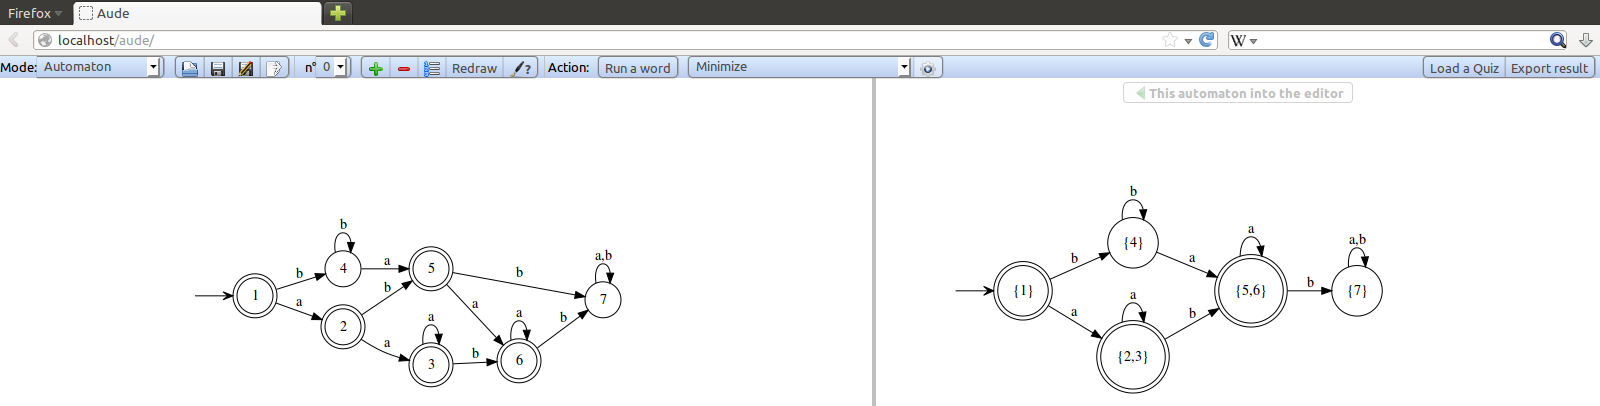
\includegraphics[width=500pt]{{../aude-algo}.png}\caption{Result of an algorithm execution.}\label{aude-algo}\end{figure}


\newpage

\paragraph{}
In addition, students can write their own algorithms using the same dedicated language as the one used for writing embedded algorithms (See figure \ref{aude-prog}).

\begin{figure}[htb]\centering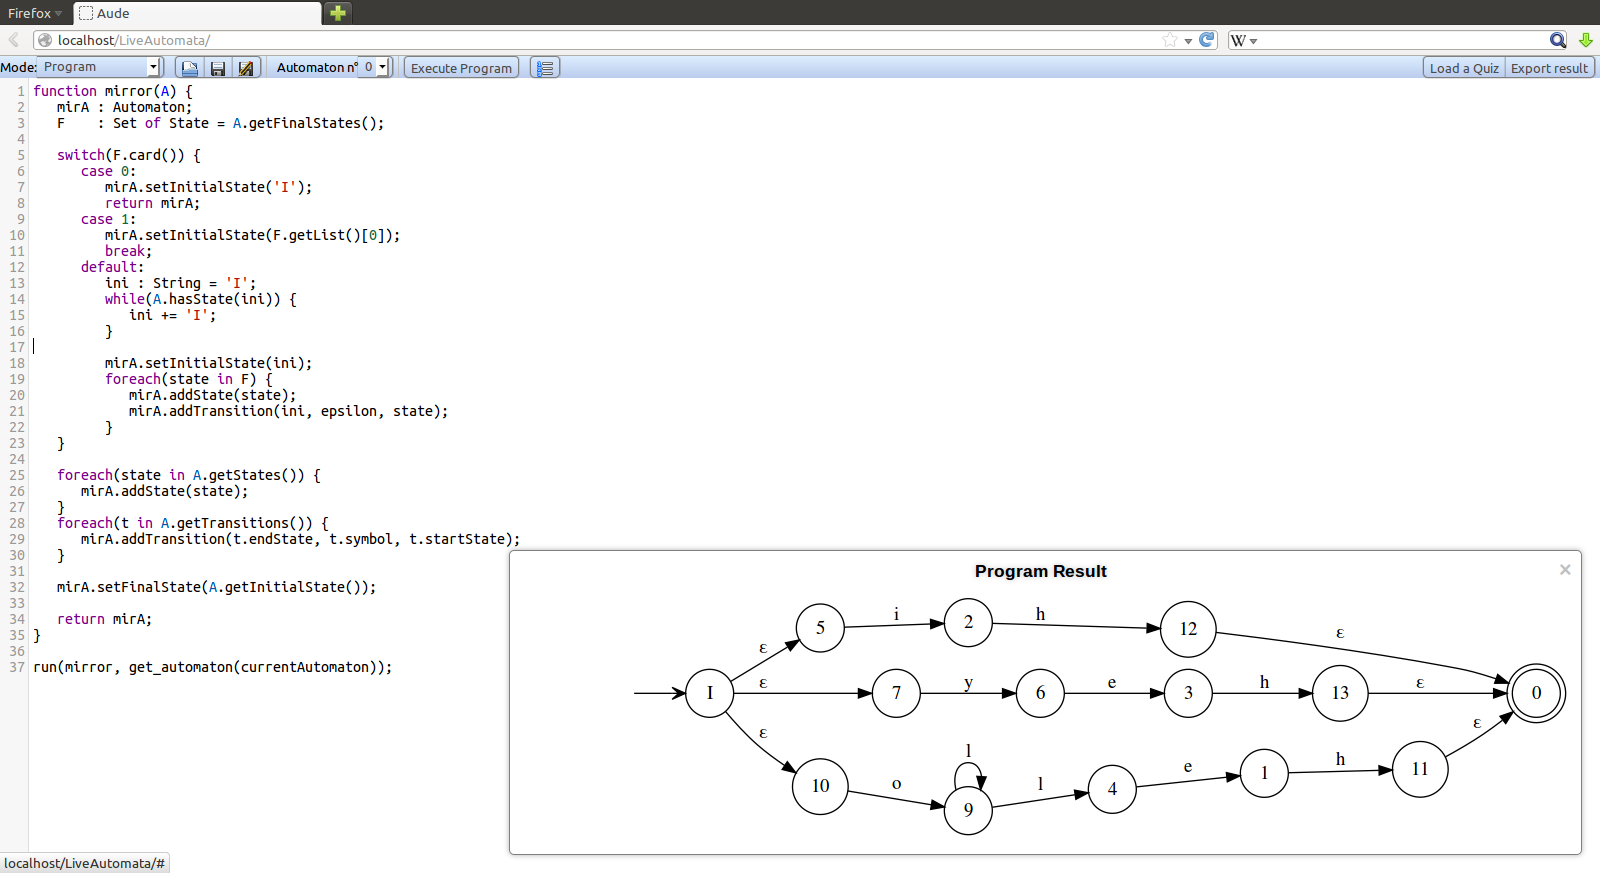
\includegraphics[width=500pt]{{../aude-prog}.png}\caption{Writing algorithms.}\label{aude-prog}\end{figure}


\paragraph{}
Algorithms can take several automata parameters. The user will be asked to choose which automata should be sent to the algorithm when running it.

    \begin{figure}[htb]\centering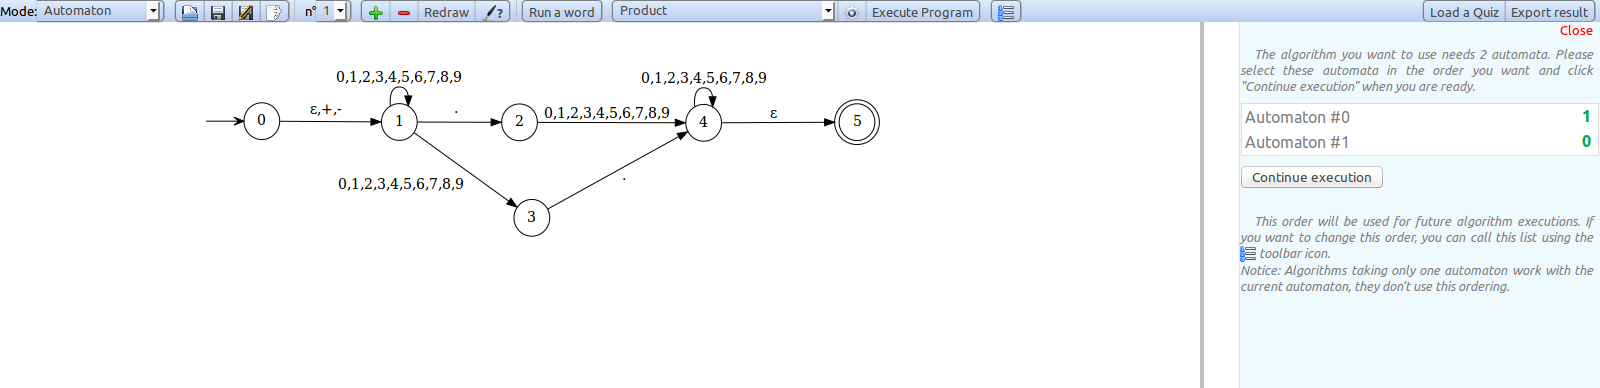
\includegraphics[width=500pt]{{../aude-list-automata}.png}\caption{Choosing which automata should be sent to the algorithm.}\label{aude-list}\end{figure}



\subsection{Running words}

\paragraph{}
Finite state automata are all about word recognition and the execution of a word is probably the most important thing to understand in the automata theory before going any farther. As a result, special care when transmitting the idea of word execution to students must be all the more taken.
The tool features animated word execution and particular attention was taken to make it easy to follow. Students can test words on their drawn and see what path(s) lead to word acceptation or from which state(s) the word was rejected (See figure \ref{word-exec}).

\begin{figure}[htb]\centering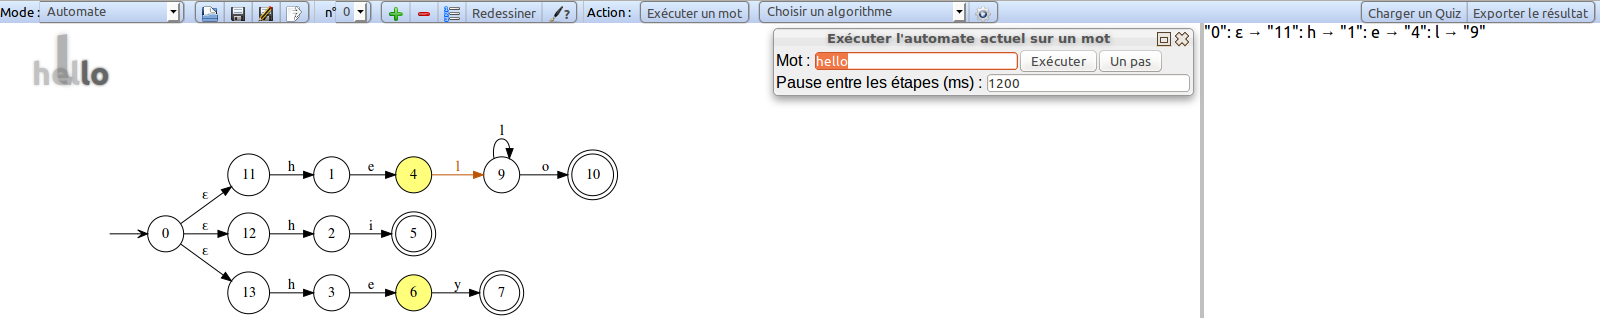
\includegraphics[width=500pt]{{../word-execution}.png}\caption{Word execution.}\label{word-exec}\end{figure}



\subsection{Quizzes}


\paragraph{}
Motivation is important, if not essential, in the process of acquiring knowledge. Interactivity sometimes helps in keeping students motivated and autonomous work can also be sought by a part of the students. \\
We tried to address the issue by implementing a Quiz module in the tool (see figure \ref{aude-quiz}). Teachers (or even students) can write custom quizzes for students so that they can train in autonomy: the tool asks questions, gathers students' responses and tell them what is right and what is wrong.

\paragraph{}
Quizzes can include:

\begin{itemize}
   \item{ mere multiple choice questions, with zero, one or more answers, with any number of possible answers.}
   \item{ questions that ask the user to draw an automaton corresponding to a set of words.}
   \item{ questions that ask the user to draw an automaton corresponding to a language defined by an automaton or a regular expression in the quiz file.}
\end{itemize}

\paragraph{}
The tool supports writing mathematics in the quiz.

\begin{figure}[htb]\centering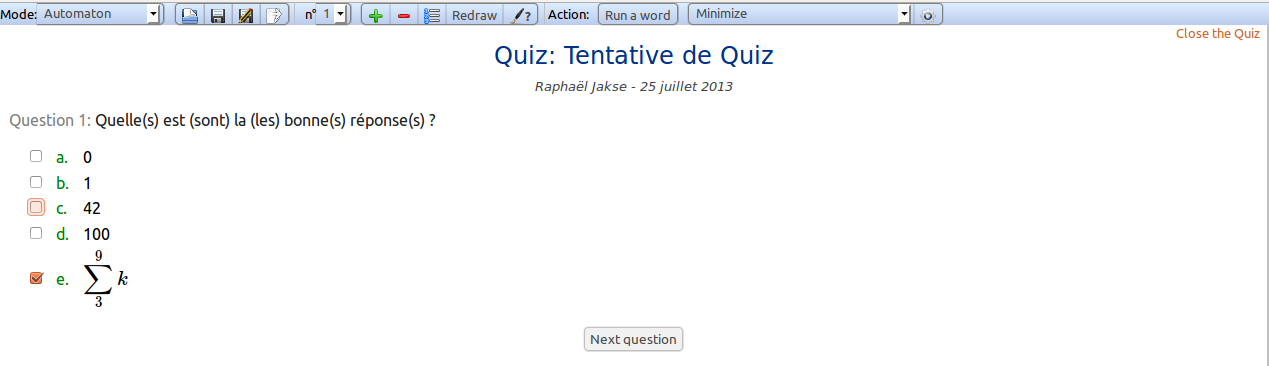
\includegraphics[width=430pt]{{../aude-quiz}.png}\caption{Quiz.}\label{aude-quiz}\end{figure}

\subsection{Automata Theory-compatible Programming Language}
\paragraph{}
The finite state automaton is usually represented by a quintuplet $(Q, \Sigma, \delta, q_0, F)$ where:
\begin{itemize}
   \item{$ Q $ is a \emph{set} of states.}
   \item{$ \Sigma $ is an alphabet. In other words, $ \Sigma $ is a \emph{set} of symbols.}
   \item{$ \delta $ is a transition relation. Put in another way, more precisely, it is a \emph{set} of triplets $(\rm{state}, \rm{symbol}, \rm{state})$.}
   \item{$ q_0 $ is the start state.}
   \item{$ F $ is a \emph{set} of states considered as final, or accepting.}
\end{itemize}

\paragraph{}
The usual definition of the finite state automaton is entirely based and completely depends on sets, and so are algorithms (see figure \ref{algo-diff})

\begin{algorithm}
   \caption{Find differentiable states}
   \label{algo-diff}
   \begin{algorithmic}
      \State \textbf{Input:} $A=(Q, \Sigma, \delta, q_{\rm{init}}, F):$ a deterministic state automaton which all states are accessible.
      \State \textbf{Output:} $D\subseteq Q \times Q$: differentiation relation between states of $ Q $
      \State \textbf{Variables:} $D, D_{\rm{pre}}, X$: sets of state couples
      \State $D \gets \left(F\times (Q \setminus F)\right)$
      \State $D_{\rm{pre}} \gets \{\}$
      \While{$D_{\rm{pre}}\neq D$}
        \State $D_{\rm{pre}}=D$
        \State $X \gets \left\{(p,q) \in Q\: | \: \exists a \in \Sigma, \left(\delta(p,a), \delta(q,a)\right) \in D\right\}$
        \State $D \gets D \cup X$
      \EndWhile
      \State \Return $D$
   \end{algorithmic}
\end{algorithm}

\lstset{language=JavaScript}

\begin{lstlisting}
function distinguableStates(A) {
   let F     = A.getFinalStates(),
       Q     = A.getStates(),
       Sigma = A.getAlphabet(),
       delta = A.getTransitionFunction(true);

   D     : Set of List = F cross (Q minus F);
   D_pre : Set of List = emptySet;
   X     : Set of List;
   while(D != D_pre) {
      D_pre = D.copy();

      X = emptySet;
      foreach(p in Q) {
         foreach(q in Q) {
            foreach(a in Sigma) {
               if([delta(p, a), delta(q, a)] belongsTo D) {
                  X.add([p, q]);
               }
            }
         }
      }

      D Union= X;
   }
   return D;
}
\end{lstlisting}

\paragraph{}
With regard to the language used for writing algorithms, we could have used Javascript directly, but Javascript is not well adapted for sets and therefore automata manipulation. The goal was to be able to write algorithms in a language which is close to their descriptions (e.g. in pseudo code), which use sets. We could have designed an entirely new language to match our expectations but that is counter-productive: it means writing a entire interpreter or compiler, which would have taken too much time and would have surely had bad performances. It would have led to an incomplete programming language to grow.

\paragraph{}
We instead opted for extending Javascript (as we already have what we need to run Javascript in a browser) with what we need: sets and some other constructions to make automata-related algorithms look better.

      
\paragraph{}
In our case, extending a programming language means:
       
\begin{itemize}
   \item{ Extending the “standard library”: adding a class to manipulate sets and a class to manipulate automata.}
   \item{ Modifying the grammar of the language: adding features like set manipulations and iteration.}
\end{itemize}

\paragraph{}
To do this, we basically need a function which takes a file written in our programming language which gives the corresponding pure Javascript code, with the following constraints:
       
\begin{itemize}
   \item{ $ n $\textsuperscript{th} line  of the generated code must correspond to the $ n $\textsuperscript{th}  line of the input code, for accuracy in error reporting}
   \item{ The generated code must be identical to the input code if the input code is pure Javascript.}
\end{itemize}

\paragraph{}
To transform the input code into pure Javascript, regular expressions come in mind, as transformations seem quite simple:
      
\noindent\begin{tabularx}{\linewidth}{|*{2}{X|}}
\hline
{\bfseries  Input code                              } & {\bfseries  Generated code (simplified)             }\tabularnewline
\hline
 \UseVerb{v1}  &  \UseVerb{v2} \tabularnewline
\hline
 \UseVerb{v3}                &  \UseVerb{v4}       \tabularnewline
\hline
\end{tabularx}

\paragraph{}
These transformations must not be done inside string literals, {\itshape object} in \lstinline!foreach! can contain parenthesis, the variable declaration can hold a initialization value, set literals look very similar to blocks of codes, \lstinline!foreach! can be nested so a need to match curly brackets appears, \lstinline!break! and \lstinline!return! statement must be transformed inside \lstinline!foreach! loop, etc. Manipulated languages are not {\itshape regular}\footnote{a language is regular iff it can be described with a regular expression. Rules like “there is the same number of opening and closing parenthesis” make a language not regular.} and transformations are not that trivial eventually. As a consequence, another method needs to be used, the code must be parsed more subtly.

\paragraph{}
A project like \href{http://zaach.github.io/jison/}{Jison}, which is a parser like \href{http://www.gnu.org/software/bison/}{Bison} might have been used\footnote{See \href{http://cjihrig.com/blog/creating-a-javascript-parser/}{http://cjihrig.com/blog/creating-a-javascript-parser/} for an implementation of a Javascript parser with Jison}. However, handwriting the parser was chosen in order to keep whitespace characters intact, to have full control over optional semicolons (if a semicolon was not written by the programmer, the semicolon should not appear in the generated code) and to handle ambiguities between regular expression tokens (which begin with \lstinline!/!) and division operators (\lstinline!/!, \lstinline!/=!) easily. Handwriting the parser also seemed to be a more efficient and straightforward solution here because transformations can be made without generating any abstract syntax tree. Moreover, this let write a quite flexible parser, validation being delegated to the actual Javascript engine, which already has a good error reporting system.
